\section{Background}

\hl{Discuss what rod cusping is and why it happens.  Show some plots from MPACT.}

\section{Traditional Solutions}

\subsection{Nodal Codes}

\hl{Discuss ways people have addressed this in the past}

\subsection{2D/1D Codes}

\hl{Discuss polynomial currently implemented in MPACT, stuff in nTRACER}

\section{Improved Decusping Methods}

\subsection{Subplane Scheme}

The subplane scheme, depicted in figure \ref{f:subplane} is a modification to the 3D CMFD acceleration discussed in section \todo{section number}.  In the traditional scheme, the MOC mesh is radially homogenized into cartesian pin cells while the axial mesh is left unchanged.  The subplane scheme changes this by allowing the homogenized coarse mesh to have multiple planes in each MOC plane.  This allows the number of MOC planes to be reduced while maintaining the accuracy and stability of a refined mesh in the axial direction.

\begin{figure}
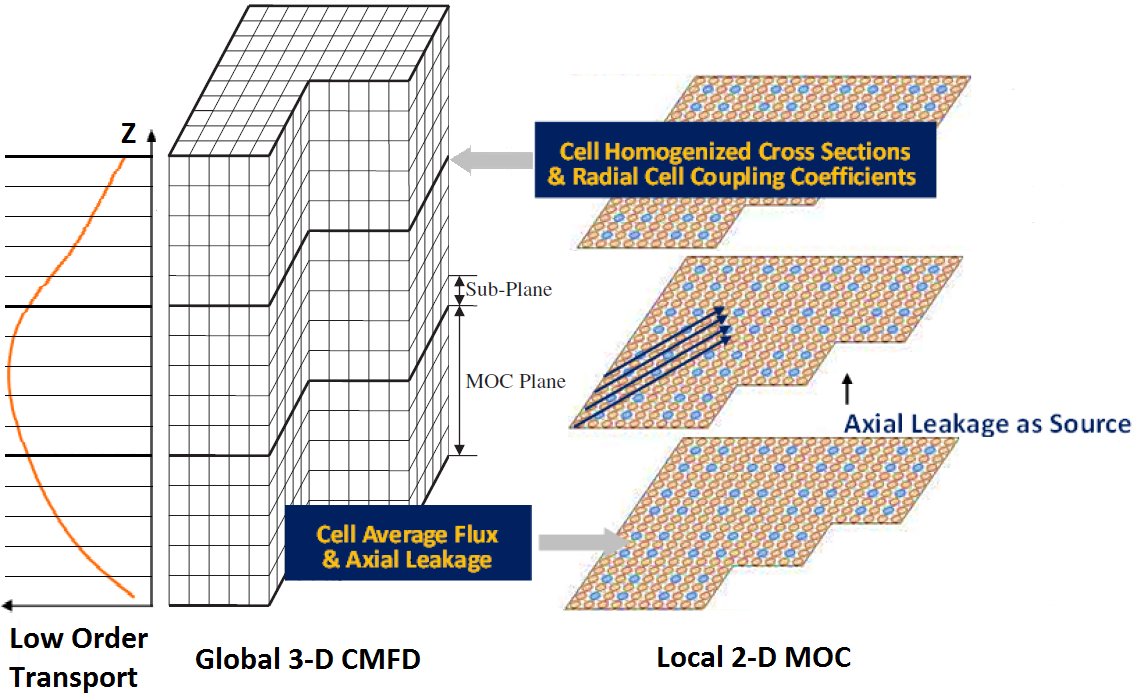
\includegraphics[width=6in]{figs/2d1d-subplane.png}
\caption{Depiction of the 2D/1D solution method with the subplane scheme}\label{f:subplane}
\end{figure}

Section \ref{ss:CMFD} discussed how to maintain consistency between the MOC and CMFD systems.  With the subplane scheme, the requirements are the same, but additional steps are needed due to the presence of additional axial planes in the CMFD system.

\subsubsection{Homogenization}

During the homogenization phase, an initial guess for the scalar flux is calculated using the previous solution:

\begin{subequations}
\begin{equation}\label{e:subplaneflux}
\phi_{CMFD,g,c}^k = \frac{\sum_{i=1}^{N_{FSR}} \phi_{MOC,g,i}^{k}V_i}{\sum_{i=1}^{N_{FSR}}V_i} c_{g,c}
\end{equation}
\begin{equation}\label{e:subplanescalingfactor}
c_{g,c}=\phi_{CMFD,g,c}^{k-1}\left(\frac{\sum_{i=1}^{N_{FSR}} \phi_{MOC,g,i}^{k-1}V_i}{\sum_{i=1}^{N_{FSR}}V_i}\right)^{-1}
\end{equation}
\end{subequations}

Volume-averaging the subplane fluxes in equation \ref{e:subplaneflux} shows that the average flux for the pin cell from the MOC solution is preserved.  The cross-sections are calculated using equation \todo{equation number}.  Because the scaling factor in equation \ref{e:subplanescalingfactor} is independent of radial position within the pin cell and the MOC flux appears in both the numerator and denominator of equation \todo{equation number}, the scaling factor cancels, giving the same cross-section as traditional CMFD system.

While the cross-sections are treated the same as for traditional CMFD, the homogenized $\chi$ values for the subplane scheme must be treated differently.  The reason for this is that the homogenized $\chi$ is fission-source-weighted instead of flux-weighted.  Because the subplane scaling factors are group-dependent and the fission source requires a sum over energy groups, the subplane scaling factor must be incorporated into the $\chi$ homogenization.  This is done using the following equations:

\begin{subequations}
\begin{equation}
\chi_{g,c} = \frac{\sum_{i=1}^{N_{FSR}} \psi_i \chi_{g,i} V_i}{\sum_{i=1}^{N_{FSR}} \psi_i V_i}
\end{equation}
\begin{equation}
\psi_{i} = \sum_{g=1}^{N_g} c_{g,c} \phi_{CMFD,g,i} \nu\Sigma_{f,g,i} 
\end{equation}
\end{subequations}

Calculating the homogenized $\chi$ using these equations ensures that the total fission source in each pin cell is preserved.

\subsubsection{Coupling Coefficients}

Finally, the CMFD system uses radial coupling coefficients calculated from the MOC solution to ensure consistency between the transport and diffusion solutions.  These coefficients are calculated as shown in equation \todo{equation number}.  When using the subplane scheme, these coefficients are needed for each subplane.  To ensure that neutron balance is preserved, the current calculated by MOC is applied to all subplanes.  Additionally, to maintain stability, the MOC flux is used to calculate the radial coupling coefficients\todo{Name the variables from whatever the CMFD equations are to make this more clear}.  This results in a constant coefficient for all subplanes in a given MOC plane.  \hl{Currently trying to change this so each subplane uses different dhats.  Should improve accuracy some, and more importantly might improve convergence.  So far, no luck.}

\subsubsection{Projection}

To project the subplane solution back to the MOC mesh, the same procedure is followed as shown in equation \todo{equation number}.  Because of the presence of multiple subplanes, the old and new CMFD fluxes are replaced with the old and new subplane-averaged CMFD fluxes:

\begin{equation}
\phi_{MOC,g,i}^k = \phi_{MOC,g,i}^{k-1} \frac{\sum_{c=1}^{N_{subplanes}} \phi_{CMFD,g,c}^k V_c}{\sum_{c=1}^{N_{subplanes}} \phi_{CMFD,g,c}^{k-1} V_c}
\end{equation}

Using this expression ensures preservation of volume-averaged flux and reaction rates in the pin cell.

\subsubsection{Results}

\todo{Add problem figures/description}

\begin{table}
\caption{Comparison of MPACT and DeCART subplane scheme results for C5G7-like rodded problem}
\begin{center}
\begin{tabular}{|l|c|c|c|c|c|c|}\hline
Plane & \multicolumn{2}{|c|}{k-eff Diff.} & \multicolumn{2}{|c|}{Max Power Diff.} & \multicolumn{2}{|c|}{Relative Runtime} \\ \cline{2-7}
Division & MPACT & DeCART & MPACT & DeCART & MPACT & DeCART \\ \hline
2 & 0.6 & 5.2 & 0.003\% & 0.04\% & 0.579 & 0.513 \\ \hline
3 & 1.9 & 7.7 & 0.004\% & 0.10\% & 0.408 & 0.327 \\ \hline
5 & 2.2 & 9.5 & 0.008\% & 0.11\% & 0.350 & 0.214 \\ \hline
10 & 1.2 & 9.8 & 0.020\% & 0.22\% & 0.253 & 0.058 \\ \hline
\end{tabular}
\end{center}
\end{table}

\begin{table}
\caption{Comparison of subplane scheme to traditional 2D/1D for VERA Progression Problem 4}
\begin{center}
\resizebox{\textwidth}{!}{\begin{tabular}{|l|c|c|c|c|c|c|c|c|}\hline
Number & k-eff Diff. & \multicolumn{2}{|c|}{Power Diff.} & \multicolumn{2}{|c|}{Outer Iterations} & \multicolumn{3}{|c|}{Runtime (core-hours)} \\\hline
of Planes & (pcm) & RMS & Max & Traditional & Subplane & Traditional & Subplane & Ratio ($\frac{Subplane}{Traditional}$) \\\cline{3-9}
32 & 0.01 & 0.001\% & 0.004\% & 29 & 30 & 21.0 & 16.2 & 0.77 \\\hline
46 & 0.01 & 0.018\% & 0.053\% & 14 & 21 & 10.3 & 8.9 & 0.86 \\\hline
62 & 0.04 & 0.023\% & 0.056\% & 12 & 20 & 12.4 & 11.5 & 0.93 \\\hline
77 & 0.04 & 0.022\% & 0.067\% & 12 & 21 & 13.0 & 11.4 & 0.88 \\\hline
\end{tabular}}
\end{center}
\end{table}

\begin{table}
\caption{Comparison of subplane scheme to traditional 2D/1D for VERA Progression Problem 5}
\begin{center}
\resizebox{\textwidth}{!}{\begin{tabular}{|l|c|c|c|c|c|c|c|c|}\hline
Number & k-eff Diff. & \multicolumn{2}{|c|}{Power Diff.} & \multicolumn{2}{|c|}{Outer Iterations} & \multicolumn{3}{|c|}{Runtime (core-hours)} \\\hline
of Planes & (pcm) & RMS & Max & Traditional & Subplane & Traditional & Subplane & Ratio ($\frac{Subplane}{Traditional}$) \\\cline{3-9}
32 & 0.01 & 0.004\% & 0.008\% & 28 & 29 & 996  & 1325 & 1.33 \\\hline
46 & 0.11 & 0.044\% & 0.111\% & 13 & 29 & 691  & 829  & 1.20 \\\hline
62 & 0.07 & 0.028\% & 0.190\% & 12 & 46 & 880  & 918  & 1.04 \\\hline
77 & 0.08 & 0.030\% & 0.184\% & 12 & 45 & 1090 & 1013 & 0.93 \\\hline
\end{tabular}}
\end{center}
\end{table}

\subsubsection{Discussion}

\begin{itemize}
\item \hl{Captures axial shape accurately with fewer planes}
\item \hl{Fewer planes means better runtime, in theory}
\item \hl{Convergence is worse.  Could be a showstopper for hard problems}
\item \hl{naturally lends itself to development of rod cusping techniques}
\end{itemize}

\subsection{Auxiliary Solvers}

The CMFD homogenized flux can be calculated as follows:

\begin{equation}\label{e:CMFDsubplaneFlux}
\phi^k_{g,c} = \frac{\sum_{i=1}^{N_{FSR}} \phi^{k=1}_{g,i} V_i}{\sum_{i=1}^{N_{FSR}} V_i} c_{g,c}
\end{equation}

The subscripts $i$, $g$, and $c$ are fine mesh cell indexes, energy group indexes, and CMFD cell indexes, respectively.  The factor $c_{g,c}$ is a group- and cell-dependent scaling factor for the subplane method.  This factor provides an axial shape to the MOC flux using the previous iterate.  It is defined as follows:

\begin{equation}\label{e:CMFDsubplaneFactor}
c_{g,c} = \frac{\phi^{k-1}_{g,c}}{\overline{\phi^k_{g,c}}}
\end{equation}

where the average flux in the denominator is defined by

\begin{equation}\label{e:CMFDaverageFlux}
\phi^k_{g,c} = \frac{\sum_{i=1}^{N_{FSR}} \phi^{k=1}_{g,i} V_i}{\sum_{i=1}^{N_{FSR}} V_i}
\end{equation}

This definition of the subplane factor provides axial shape while still preserving the volume-averaged flux and reaction rates in each pin cell in the MOC plane.

The CMFD homogenized cross-sections can be calculated using the MOC flux:

\begin{equation}\label{e:CMFDhomXS}
\Sigma_{x,c} = \frac{\sum_{i=1}^{N_{FSR}} \phi_{g,i}\Sigma_{x,g,i}V_i}{\sum_{i=1}^{N_{FSR}} \phi_{g,i}V_i}
\end{equation}

Multiplying equations \ref{e:CMFDsubplaneFlux} and \ref{e:CMFDhomXS} gives the reaction rate in the pin cell.

When using the embedded solver, a radial flux profile is obtained from the solver.  The process described above is followed for the nodes around the partially inserted rod.  However, instead of the MOC flux, the radial flux from the embedded solver is used.  This allows subplanes with partially inserted control rods to have different cross-sections based on the radial flux profile around the tip of the control rod.

\hl{The flux coming out of the embedded solver is treated as a shape function and scaled to preserve the MOC flux.}

\hl{Need to make sure reaction rates are preserved I think}.

\hl{A constant current is used for all subplanes.  This does not provide the most accurate solution, but ensures stability and neutron balance.}

\hl{When projecting, the subplane fluxes scale MOC fluxes.  Reference equation.}

\hl{The cross-sections can be modified by mixing the rodded and unrodded cross-sections.  Equation from Han Joo cusping paper.}

\section{Future Work}

\begin{itemize}
\item \hl{Improved shape for dhats in sublpane (without sacrificing stability)}
\item \hl{New ``sub-ray'' MOC}
\item \hl{Radial shape for axial TL source (ref. Mike Jarrett)}
\end{itemize}